\fancyhead[LO, RE]{Augmenter les sources d'analyse}

Une analyse efficace et intéressante nécessite une diversité de textes pour accroître nos résultats et leur hétérogénéité. Le seul élément d'analyse à disposition au commencement du stage se compose du chapitre 30/31/36, transcris antérieurement au début du stage et si notre corpus se compose effectivement de nombreuses versions du \emph{Traité}\index{Traite des delits et des peines@Traité des délits et des peines} de Beccaria, cela représente majoritairement toujours les mêmes éléments. Il est donc essentiel d'augmenter nos sources d'analyses pour observer les résultats sur un chapitre du même corpus mais d'un sujet différent.

Parmi les premières réflexions faites pendant l'atelier de février et la première réunion avec les responsables du projet, l'idée d'utiliser certains chapitres plutôt que d'autres a été avancée et après relecture du traité\index{Traite des delits et des peines@Traité des délits et des peines} et considération des différents chapitres, le choix s'est porté sur l'introduction, accompagné des trois premiers chapitres (\og~Origine des peines~\fg{}, \og~Droit de punir~\fg{}, \og~Conséquences~\fg{}) et sur le chapitre 7/13/14 (en fonction des versions) qui porte sur les \og~Indices et formes de jugements~\fg{}. Ce dernier chapitre semblait pertinent, car il porte sur du droit mais dans un contexte un peu différent du chapitre 30/31/36 pour lequel se fait déjà l'analyse. Il y aurait donc de l'intérêt à apporter d'autres éléments et résultats d'analyse vis-à-vis des termes clés et du langage juridique.

Une fois ces chapitres sélectionnés, plusieurs étapes sont nécessaires pour obtenir la version transcrite propre que nous modifierons par tous les scripts de nettoyage de texte.

\section{Méthodes pour la transcription automatisée de la source}
La \acrfull{ocr}\index{OCR} consiste à convertir l'image d'un texte en un texte lisible électroniquement, en faisant le moins de fautes possible lors de la conversion. L'objectif avec ces outils a longtemps été d'obtenir une reconnaissance parfaite, sans erreur, mais cela est compliqué et oblige à prendre en compte divers critères pour optimiser l'utilisation du système d'\acrshort{ocr}\index{OCR} avec le document. 

\subsection{Aider à l'océrisation}
Au fur et à mesure de l'utilisation de ces logiciels d'\acrshort{ocr}\index{OCR}, il a été observé qu'il était nécessaire de pré-traiter le document qui sera océrisé pour optimiser l'utilisation du logiciel tel qu'en opérant un \og~débruitage~\fg{} ou un redressement d'image. Des applications se sont développées pour opérer en amont ce genre de correction et avoir ainsi un texte à disposition prêt à être manipulé par l'\acrshort{ocr}\index{OCR}\footnote{Exemple de \emph{ScanTailor}~: \url{https://github.com/scantailor/scantailor}}. Une autre des aides apportées à l'efficacité de la conversion est le paramétrage de certains des moteurs d'\acrshort{ocr}\index{OCR} pour qu'ils sachent prendre en compte les particularités qui pourraient se présenter dans le document texte. Il existe une multitude de textes qui nécessitent des océrisations\index{OCR!ocerisation@océrisation} et qui ne sont pas simplement des textes dactylographiés~: il faut tenir compte des langues, des spécificités d'écriture ou bien même de la mise en page du texte, ce qui nécessite une couche supplémentaire de réflexions du logiciel d'\acrshort{ocr}\index{OCR} si le texte contient une quelconque particularité, tel que des caractères nouveaux et inconnus ou une police d'écriture d'un style compliqué, tel que cela s'observe pour le cas de l'allemand dans notre analyse.

\subsection{Entraînement du système~: apprentissage automatique des caractères}
La reconnaissance optique des caractères consiste en la lecture d'une image d'un texte menant à une identification de sa composition, pour ressortir alors une version écrite de ce texte. Cela nécessite un travail en amont de programmation du logiciel et si diverses méthodes ont été autrefois utilisées pour mener à bien ce travail, la principale, considérée également comme la plus efficace, repose aujourd'hui sur le \textit{machine learning} ou apprentissage automatique. Cela consiste en un entraînement fourni au logiciel qui devra océriser\index{OCR!ocerisation@océrisation}, pour qu'il ait la capacité de reconnaître les caractères qu'il lit. Par le biais de multiples données et documents mis à sa disposition, le logiciel s'entraîne à reconnaître ce qui lui est soumis et crée alors des modèles de caractères. 
Certains logiciels peuvent ensuite aller plus loin en travaillant avec des réseaux de LSTM ou \textit{Long Short-Term Memory}. Cela consiste à travailler un document à travers une chaine d’informations et à s’adapter et à prendre en compte les données rencontrées au fur et à mesure. Lors du travail de la chaine, des informations peuvent être ajoutées ou supprimées dans le modèle de données, afin de toujours le mettre à jour\footnote{\url{http://colah.github.io/posts/2015-08-Understanding-LSTMs/}}. Une fois que le système d'\acrshort{ocr}\index{OCR} a à sa disposition les modèles compétents et adaptés pour réaliser sa tâche, il est possible de lancer le processus d'océrisation\index{OCR!ocerisation@océrisation} et ses différentes étapes, qui permettent d'effectuer la transformation.


\subsection{Déconstruction de l'OCR}
La chaîne de transcription est composée de trois étapes ordonnées~: la segmentation, la reconnaissance de textes et le post-traitement. 

La segmentation consiste en l'analyse de la structure des pages ainsi qu'en la recherche des structures de textes et des blancs dans l'image pour pouvoir reconnaître les zones de textes. Le logiciel repère les éléments dans la page qu'il devra prendre en compte pour la suite de son processus, il repère les caractères typographiques et la mise en page des textes et une fois cela fait, il cherche l'ordre au milieu de tout ça, pour qu'il sache d'avance comment cela devra basiquement se présenter. En fonction des algorithmes choisis, cela peut s'effectuer en partant des caractères pour aller jusqu'au niveau de la page, ou à l'inverse en partant de la page en son entier pour plonger dans l'image jusqu'aux caractères. 

Une fois ces informations récupérées, le logiciel d'\acrshort{ocr}\index{OCR} procède à la reconnaissance de caractères, c'est-à-dire qu'une fois que la zone de texte est repérée, le système lit les caractères qui sont inscrits et il les compare aux banques de données de caractères qu'il a à sa disposition pour ressortir le bon et pouvoir ensuite former un mot avec ce caractère et ceux qu'il aura identifié à proximité. Cela peut être ardu, notamment dans le cas où les alphabets ne sont pas les mêmes ou si certains caractères ne se présentent pas toujours de la même façon. Cette tâche pourra être supportée par une des étapes du prétraitement qui consiste à établir certains paramètres. Il saura ainsi plus aisément ce qu'il cherche et identifiera plus facilement les caractères puis les mots.

Après que le système ait reconnu les caractères du document papier et ait commencé à former des mots, l'étape du post-traitement est lancée. L'étape précédente a formé une liste de propositions pour chaque mot par ordre de vraisemblance et cette étape a pour but de les analyser pour vérifier quel mot correspond le plus et surtout diminuer le nombre d'erreurs dans la transcription. Le post-traitement s'appuie sur des corrections orthographiques et morphologiques ainsi que syntaxiques à l'échelle de la phrase. Les logiciels, en fonction de leur programmation, peuvent également se baser sur leurs connaissances linguistiques, en observant les spécificités du texte qu'ils ont à portée, ou pragmatiques, en examinant le contexte du document et la place des phrases, pour voir par exemple si le caractère est une majuscule ou non.

Ces trois étapes permettent d'aboutir à un texte transcrit plus ou moins correctement, mais certains possèdent des fautes récurrentes non corrigeables, car les systèmes d'\acrshort{ocr}\index{OCR} ont des limites qui n'ont pas encore pu être dépassées et qui restent attachées à certains types de textes.

\subsection{Difficultés récurrentes du processus}
La méthode d'\acrshort{ocr}\index{OCR} s'est considérablement développée et ne se base plus sur une idée de réussite à 100\% de la transcription, ce qui est presque impossible, même si la mise en place de nombreux paramètres permet de se rapprocher un peu plus de cette perfection. 

Malgré ces progrès, on retrouve certaines erreurs récurrentes, qui peuvent être plus présentes en fonction du type de document à disposition. Trois types d'erreurs peuvent principalement être observées et elles sont rattachées chacune à une des étapes du processus d'\acrshort{ocr}\index{OCR}. Il peut tout d'abord y avoir les erreurs de segmentation, qui prennent plusieurs formes et se matérialisent généralement par une mauvaise lecture de la structure de texte~: des zones de lecture sont fusionnées, certaines sont séparées, l'ordre de lecture est mélangé, etc. On trouve ensuite les erreurs de reconnaissance de caractères, qui sont divisées en quatre~: confusion (un caractère remplacé par un autre), suppression (caractère considéré comme du bruit donc non reproduit), rejet (caractère non reconnu donc non inscrit) et ajout (caractère dédoublé par deux autres car forme proche). Enfin, avec la dernière étape vient la dernière erreur, une erreur de reconnaissance de mots~: une mauvaise qualité de l'image peut apporter des difficultés de lecture au processus qui interprétera mal certains espaces dans le texte et créera une scission dans un mot ou alors fusionnera deux mots ensemble. En plus de ces erreurs, il existe aujourd'hui certains textes qui sont toujours difficiles à travailler, notamment les manuscrits anciens et patrimoniaux, ceci étant dû à des obstacles typographiques et physiques des documents pour le logiciel d'\acrshort{ocr}\index{OCR}\footcite{bensalah_mass_digitization}\footcite{belaid_numerisation}.

Cependant, devant l'utilisation de plus en plus fréquente des processus d'\acrshort{ocr}\index{OCR} et sur des textes de plus en plus volumineux, ont été créés des applications et des systèmes qui essaient a posteriori de gommer ces erreurs, pour obtenir un texte plus propre et plus exact. On peut citer à ce propos le projet AméliOCR, \og~dont l'objectif est d'améliorer la qualité du texte dans les documents historiques numérisés au sein de la bibliothèque numérique Gallica~\footcite{chiron_erreurs_ocr}\fg{} ou bien même une compétition qui s'est tenue en 2017, la compétition Post-OCR Text Correction qui avait pour but de présenter ces fameux systèmes et d'élire le meilleur\footcite{magallon_erreurs_ocr}.

\section{Obtenir les images pour l'océrisation~: convertir les PDF de texte}
Pour pouvoir passer des fichiers par le script d'\acrshort{ocr}\index{OCR} afin d'obtenir les versions transcrites de nos chapitres, il faut tout d'abord trouver un moyen d'obtenir ces fichiers de manière adéquate et adaptée au script. Il n'est pas possible de passer tout le \textsc{pdf} par le script d'\acrshort{ocr}\index{OCR}, tout d'abord parce que ce n'est pas là le but recherché (nous souhaitons seulement deux extraits du \textit{Traité}\index{Traite des delits et des peines@Traité des délits et des peines}) et ensuite car le script n'est pas adapté au \textsc{pdf}, notamment parce que ce sont plusieurs pages dans un seul fichier, alors que l'\acrshort{ocr}\index{OCR} transcrit par une page/un fichier. Il est donc nécessaire d'opérer une conversion sur les \textsc{pdf} pour les obtenir découpés et avec une extension .tif ou si nécessaire, .jpg.

\subsection{Extension TIFF~: une image plus nette et plus adaptée}
Le choix principal pour convertir les \textsc{pdf} est celui d'une extension \textsc{tiff} car elle présente quelques avantages qui la rendent préférable pour l'exploitation \acrshort{ocr}\index{OCR}. En effet, le format \textsc{tiff} garde la taille de base de l'image et donc par extension, la qualité de l'image, ce que nous n'aurons pas avec \textsc{jpeg}, qui est un format de fichier \og~à perte~\fg{} c'est-à-dire que le fichier est moins lourd mais cela produira une moindre qualité de l'image. Ce problème est conséquent dans le cas de notre utilisation, puisque nous souhaitons utiliser le fichier pour l'océriser. Pour pouvoir espérer avoir un bon résultat, avec un texte fidèle à ce qui est écrit sur l'image, nous devons donner au script Python le meilleur fichier possible. Ainsi, le fichier \textsc{tiff} sera possiblement assez lourd mais offrira une meilleure lisibilité, parfaite pour son exploitation.

Pour obtenir ce fichier \textsc{tiff}, nous utilisons un extracteur d'images, qui est lié à Linux et qui fonctionne en ligne de commandes~: \emph{PDFImages}. Ce module permet d'extraire le contenu de n'importe quel fichier \textsc{pdf} pour les transformer avec l'extension voulue. Il propose de nombreuses extensions de fichiers pour la conversion, comme notamment \textsc{tiff} et \textsc{jpeg} et offre aussi la possibilité d'insérer des options dans l'invite de commande, pour faire apparaître les détails voulus. Notre utilisation est plutôt basique pour le cas de la conversion, puisqu'il sera simplement spécifier l'extension de fichier, le fichier d'entrée et le dossier de sortie, sans insérer plus d'options. Il est alors obtenu la conversion de notre \textsc{pdf} en une multitude de fichiers \textsc{tiff}, un pour chaque page, qui ont chacun une taille conséquente (les \textsc{jpeg} font entre 3 et 7 Mo, alors que les \textsc{tiff} sont réguliers avec environ 6 à 7 Mo par fichier), montrant que l'ensemble des images sera probablement de bonne qualité.

Nous verrons par la suite que le format \textsc{tiff} offre également un autre aspect pratique pour la future océrisation\index{OCR!ocerisation@océrisation} du fichier, aspect non disponible pour les \textsc{jpeg}, que nous allons également devoir utiliser, à cause de certaines particularités de fichiers \textsc{pdf} vis-à-vis des \textsc{tiff} lors de la conversion.

\subsection{Extension JPEG~: une solution de secours moins performante}
L'extension \textsc{jpeg}, comme nous l'avons vu, est un fichier qui fait perdre de la qualité à l'image lorsque la conversion s'opère mais qui s'avère impératif à utiliser pour certaines éditions en \textsc{pdf} du traité\index{Traite des delits et des peines@Traité des délits et des peines}. Effectivement, lors de la conversion de tous les fichiers \textsc{pdf} en \textsc{tiff}, deux types de résultats sont observés~: soit le document est converti correctement et il y a tout l'ouvrage page par page, soit le convertisseur rencontre une difficulté dans la lecture du document et extrait chaque page de trois manières différentes (une présentation brouillon et illisible de la page, la page de texte en négatif, avec un texte blanc sur noir et la version vierge de la page sur lequel est écrit le texte), ce qui est illustré dans la figure \ref{fig:resultatTIFF}. 
\begin{figure}[p]
    \centering
    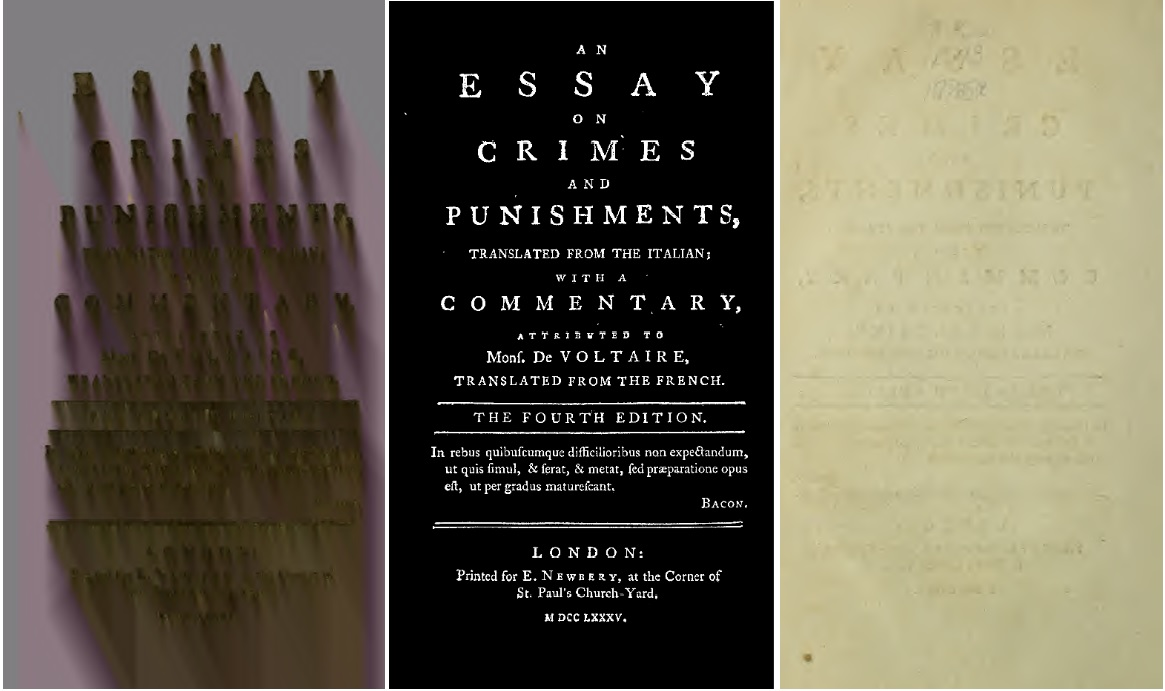
\includegraphics[width=15cm]{Partie2/images/Resultat_TIFF.jpg}
    \caption{Résultat d'une océrisation\index{OCR!ocerisation@océrisation} en \textsc{tiff} pour l'édition anglaise de 1785 du Beccaria}
    \label{fig:resultatTIFF}
\end{figure}

Dans le cas où est obtenu ce second résultat, cela pose un problème pour la suite, puisque si cela est effectivement possible de récupérer le deuxième type de production (le texte en négatif) et qu'il peut parfois être exploitable, la majorité du temps, cela s'avère peu lisible pour le script d'\acrshort{ocr}\index{OCR}, qui ne sait pas exactement ce qu'il est censé aller chercher et les résultats sont généralement assez mauvais et inutilisables.
\begin{figure}[p]
    \centering
    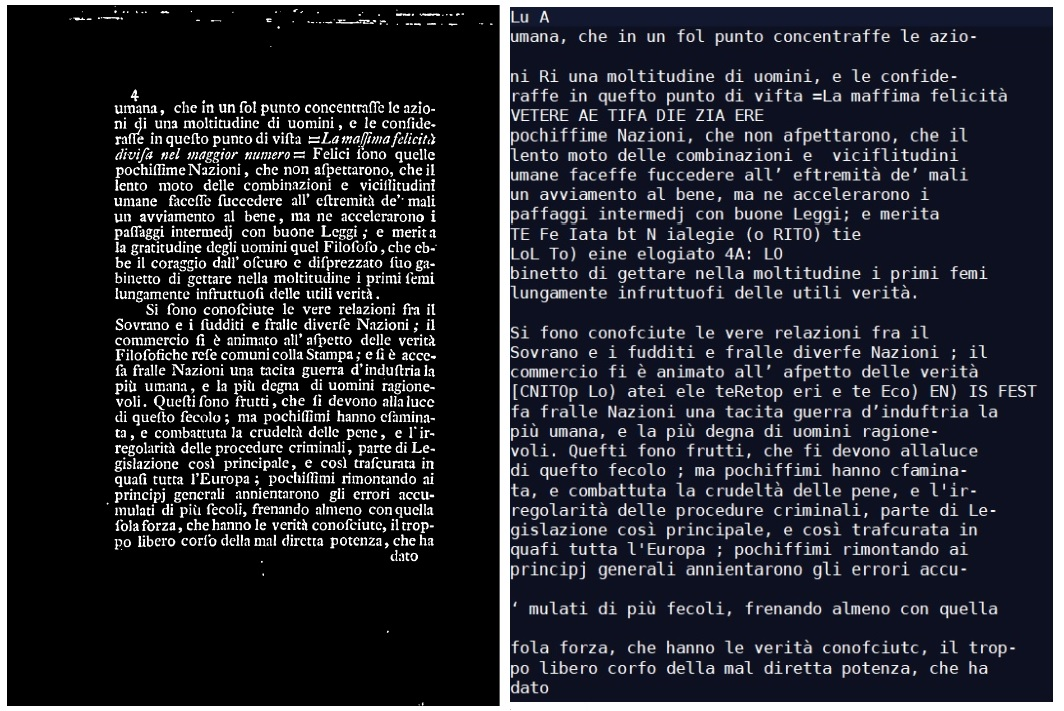
\includegraphics[width=15cm]{Partie2/images/BadTranscript_TIFF.jpg}
    \caption{Mauvaise transcription de texte, dû à l'aspect de l'image numérisée}
    \label{fig:badtranscript}
\end{figure}
Lorsque ce cas se présente, comme dans la figure \ref{fig:badtranscript}, il est donc nécessaire de produire les fichiers dans un format \textsc{jpeg}, en espérant que le document soit assez lisible pour l'\acrshort{ocr}\index{OCR} et qu'il produise un meilleur texte que le négatif du \textsc{tiff}.

Pour faire cette transformation, j'ai utilisé l'application \emph{\textsc{pdf} to \textsc{jpeg}}, qui est un convertisseur Windows, où il suffit de lui donner le fichier d'entrée, soit le fichier \textsc{pdf} à convertir, de lui donner un lieu de sortie, soit le dossier où il devra ranger les pages converties en \textsc{jpeg}. Ensuite, nous lui faisons convertir et l'opération dure entre 30 secondes et 3 minutes. Cette technique est aussi pratique que celle du \emph{PDFImages}, bien qu'elle ne soit disponible qu'en \textsc{jpeg} et seulement sur Windows. L'image est tout de même réduite et perd de la qualité, comme cela s'observe en essayant de l'agrandir pour avoir une meilleure résolution. Nous voyons que cela est très limité pour les \textsc{jpeg}, alors que cela peut se faire beaucoup plus facilement avec les \textsc{tiff}. Cela reste une option à avoir, puisque lors de la correction de la transcription, il peut être essentiel, dans le cas d'un caractère un peu effacé ou d'un mot difficile à lire, d'agrandir l'image pour mieux voir ce qui est écrit.

\paragraph{} Le \textsc{jpeg} est donc plus limité que le \textsc{tiff} pour la lecture et l'utilisation de fichiers et même s'il est utilisé pendant notre démarche, il donne lieu à un travail plus long dans la correction de la transcription puisque cela demande de corriger plus d'éléments dans le texte et d'être encore plus précis que d'habitude. De plus, le \textsc{jpeg} est plus problématique à utiliser que le \textsc{tiff}, car il n'est pas compatible, sur la plupart des ordinateurs, avec \emph{ScanTailor}, outil qui aura une fonction notable avant l'océrisation\index{OCR!ocerisation@océrisation} pour les fichiers \textsc{tiff}.

\section{Étape intermédiaire~: nettoyer ses images pour un meilleur fichier source}
Lorsque nos chapitres sont composés de fichiers avec une extension \textsc{tiff}, nous avons la possibilité d'effectuer une étape intermédiaire, qui permet d'améliorer le fichier qui sera soumis au script python pour océriser les images.

Les images en \textsc{tiff} peuvent être nettoyées partiellement à l'aide d'un logiciel~: \emph{ScanTailor}. Cette application se compose de multiples options pour pouvoir manipuler l'image et la rendre plus claire et mieux lisible par le processus d'océrisation\index{OCR!ocerisation@océrisation}. Le nettoyage se déroule en cinq étapes (la cinquième comptant elle-même plusieurs manipulations). L'image peut être scindée, dans le cas où il y a deux pages ensemble et que nous ne voulons avoir qu'une page à traiter individuellement pour la suite~; puis elle peut être redressée, dans le cas où l'écriture n'est pas droite et le texte doit être quelque peu relevé ou descendu~; ensuite, se choisit le contenu que nous voudrons faire lire par la suite. Dans un cas où nous ne voulons pas tout le texte présent sur la page mais seulement un extrait, il est possible de sélectionner ce contenu précis et à la fin, le logiciel supprimera le reste sur la page manipulée. Par la suite, nous pouvons définir les marges et enfin, la cinquième étape sera celle de la sortie. L'application produit l'image telle que nous lui avons demandée de nous la présenter durant toutes les étapes présentées et il est encore faisable d'effectuer certaines modifications. L'image est produite directement en noir et blanc, mais il est possible de revenir à la version précédente avec la coloration originale de la page. Le noir et blanc est pratique notamment car il permet d'être mieux lu par l'\acrshort{ocr}\index{OCR}. Nous pouvons également décider d'augmenter le niveau d'encre pour l'écriture, ce qui est une option utile dans le cas où le texte est un peu effacé (ce renforcement donnera la possibilité de lire certains mots peu ou non apparents précédemment). Enfin, avec cette sortie, peut également s'utiliser une fonction \og~balayage~\fg{} qui nettoie notre page, c'est-à-dire qu'elle enlève les points présents sur les pages, les ratures, ou les dégradations un peu voyantes du papier. Cela a tout de même une limite puisque l'option de balayage est disponible en plusieurs niveaux et parfois, les niveaux les plus élevés enlèvent des éléments nécessaires, comme les numéros de page ou même parfois des bouts de texte.

Les images modifiées par cette application ressortent ainsi plus claires, débarrassées de presque tout ce qui pouvait entraver la bonne lecture et la bonne transcription des caractères et donc le fichier est prêt pour être océrisé et ainsi produire un texte brut.

\section{Étape finale~: océrisation et nettoyage du texte}
Une fois toutes les manipulations faites pour obtenir une image unique numérisée avec une extension exploitable par un logiciel \acrshort{ocr}\index{OCR} et plus ou moins nettoyée pour un meilleur usage, la transcription pour produire un fichier texte peut s'effectuer, qui nous donnera, une fois tous les fichiers texte réunis et nettoyés, un chapitre complet transcrit.

\subsection{Préparer l'OCR~: installation et programmation de \emph{Tesseract}}
\subsubsection{Choisir son module d'OCR}
Le processus d'océrisation\index{OCR!ocerisation@océrisation} est aujourd'hui très répandu, pour de très nombreux types d'utilisation. Cette expansion de la méthode a permis la création de très nombreux logiciels d'\acrshort{ocr}\index{OCR}, disponibles en open source, comme \emph{Kraken}, \emph{Calamari} ou \emph{Tesseract}, ou non, pour des sources matérielles courtes ou inversement de très longs documents comme \emph{Google Cloud Vision} ou \emph{Microsoft Azure Computer Vision} et qui peuvent avoir un usage professionnel ou personnel. Des études ont été faites pour démontrer les différences entre ces logiciels et savoir lesquels fonctionnent le mieux en fonction de l'utilisation faite ou de la source matérielle{\footnote{\url{https://source.opennews.org/articles/so-many-ocr-options/ }}}.

Dans le cas de nos travaux, nous avons décidé d'utiliser \emph{Tesseract}{\footnote{\url{https://github.com/tesseract-ocr/tesseract}}} pour océriser les nouveaux chapitres du \textit{Traité}\index{Traite des delits et des peines@Traité des délits et des peines} de Beccaria. \emph{Tesseract} a l'avantage d'être open source et surtout d'être utilisable en ligne de commande (nous avons donc la possibilité de l'utiliser avec Python, notre outil de programmation depuis le début du travail). De plus, \emph{Tesseract} est très bien documenté sur sa page Github et il est donc possible d'installer tout ce qui est nécessaire, et notamment des spécificités, qui vont être nécessaires dans le cas de nos transcriptions de Beccaria. Ces spécificités sont notamment indispensables car \emph{Tesseract} fait partie des logiciels d'\acrshort{ocr}\index{OCR} qui n'ont pas de modèles préexistants dans sa programmation. Il faut donc les installer en plus de l'installation du logiciel \emph{Tesseract}. Nous utilisons \emph{Tesseract} avec \emph{PIL (Python Imaging Library)}, une bibliothèque de traitements d'images (faisant partie des librairies Python), qui permet un accès rapide aux données contenues dans une image et pour plusieurs types d'extensions d'images.

\subsubsection{Installer le logiciel \emph{Tesseract}}
Une fois le logiciel choisi, il suffit de suivre les instructions inscrites sur le Github pour installer \emph{Tesseract}. Étant sur un terminal Linux, il suffit de taper la commande \textit{\og~sudo apt install tesseract-ocr~\fg{}} et le logiciel est installé mais pas encore prêt pour utilisation. En effet, il est nécessaire, pour que \emph{Tesseract} fasse ce qui lui est demandé, d'installer également les langues à traiter avec l'\acrshort{ocr}\index{OCR}. Dans notre cas, cela sera l'italien, le français, l'anglais et l'allemand et nous devrons donc installer quatre langues sur \emph{Tesseract}. En réalité, cinq installations sont nécessaires pour avoir tous les éléments d'une bonne océrisation\index{OCR!ocerisation@océrisation}.

Tout d'abord, s'installera l'italien, le français et l'anglais, qui ne posent aucun problème~:
\begin{itemize}
    \item sudo apt install tesseract-ocr-ita (italien)
    \item sudo apt install tesseract-ocr-fra (français)
    \item sudo apt install tesseract-ocr-eng (anglais)
\end{itemize}
Il faudra cependant faire deux installations pour l'allemand~:
\begin{itemize}
    \item sudo apt install tesseract-ocr-deu
    \item sudo apt install tesseract-ocr-frk
\end{itemize}
Nous installons l'allemand standard, qui sera utile pour quelques traductions mais également l'allemand \emph{fraktur}, qui aura la possibilité de reconnaître, pendant l'océrisation\index{OCR!ocerisation@océrisation}, qu'il n'est pas en présence d'un texte allemand écrit de manière standard mais d'un texte allemand rédigé avec l'écriture \emph{fraktur}, plus difficile à reconnaître et à lire qu'un alphabet standard. Cela implique donc que \emph{Tesseract} doit être programmé pour pouvoir reconnaître ces caractères, sinon il est très probable qu'il ne sache lire que très difficilement les textes lorsqu'ils sont écrits ainsi. Il est possible par la suite, installer d'autres langues, dans le cas où des traductions d'éditions dans d'autres langues sont découvertes et insérées dans notre projet.

\subsection{Application du script d'OCR}
Nous avons deux scripts \acrshort{ocr}\index{OCR}, un pour l'extension \textsc{tiff} et un pour l'extension \textsc{jpeg}, mais ils ne sont pas fondamentalement différents, seul un élément change entre les deux impactant ainsi leur mode de fonctionnement. Le script est rédigé de manière à ce que l'invite de commande aille chercher les images, les lise, en extrait le texte qu'il visualise et l'inscrit dans un nouveau document ayant le même nom que l'image qu'il traite mais avec une extension \textsc{txt}.
\begin{figure}[t]
    \centering
    \fbox{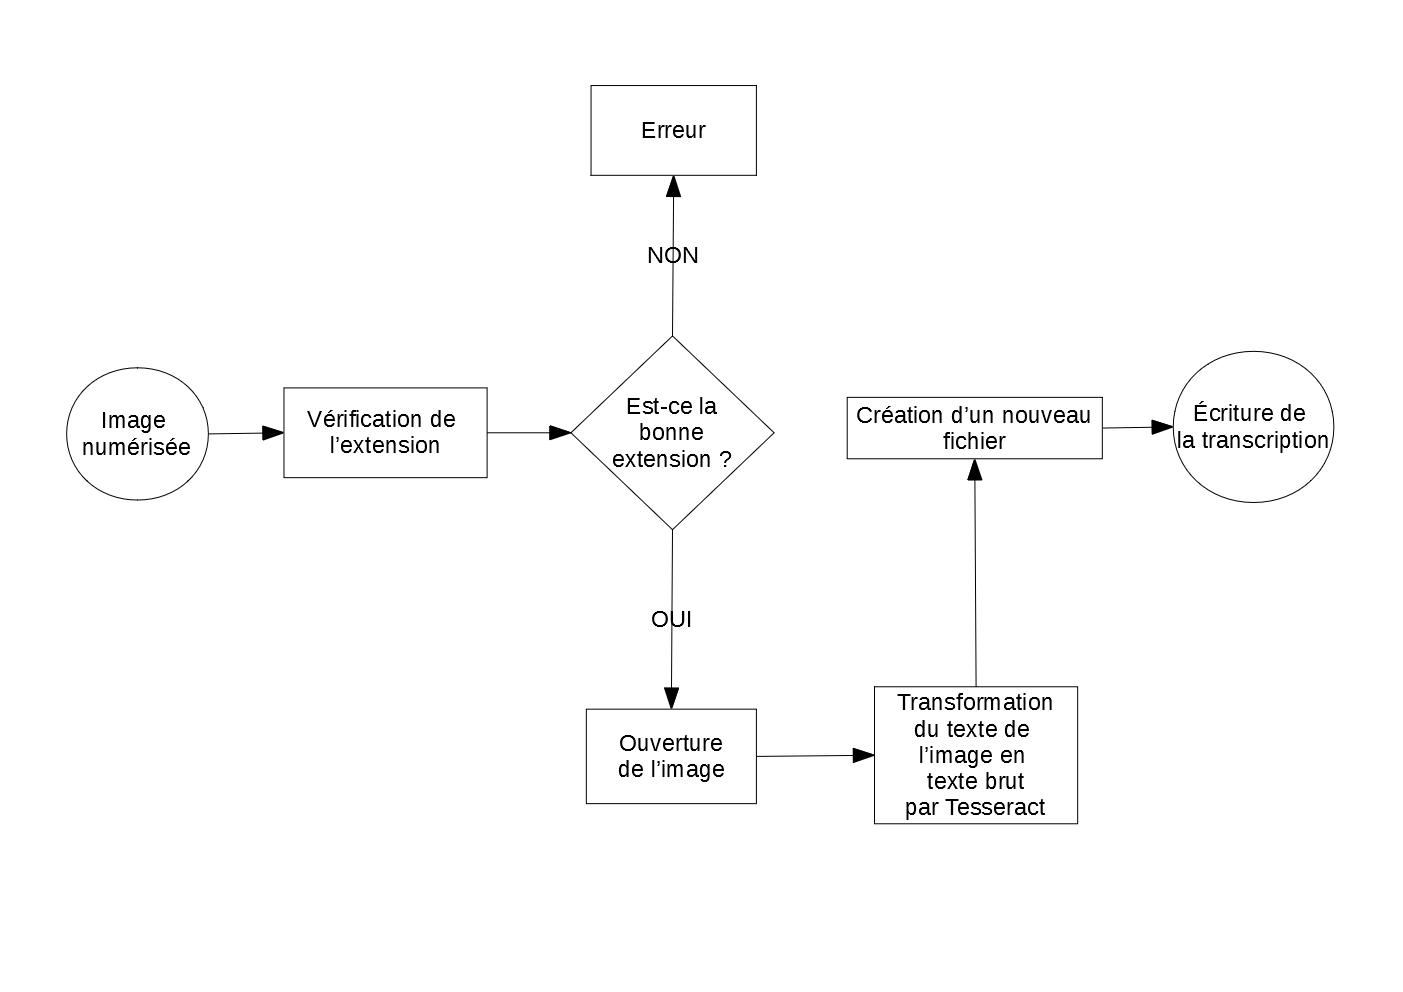
\includegraphics[width=16cm]{Partie2/schemas/OCR.jpg}}
    \caption{Étapes de la transcription, d'une image numérisée à un fichier texte brut}
    \label{fig:OCR}
\end{figure}
La différence entre \textsc{tiff} et \textsc{jpeg} est le fait que nous demandons à l'invite de commande d'aller chercher les images numérisées et il est spécifié dans le script que pour reconnaître la source matérielle, le terminal doit trouver une extension définie pour savoir quel document traiter, et c'est donc à la première ligne de la boucle \textit{for} que s'effectue le changement~:
\begin{itemize}
    \item \mint{python}{if i.endswith("jpg"): (pour ocr_jpg.py)}
    \item \mint{python}{if i.endswith("tif"): (pour ocr_tiff.py)}
\end{itemize}
Ainsi, avec cette différence, nous pouvons traiter soit les images qui sont passées sans problème par la conversion en \textsc{tiff}, soit celles qui ont dû passer par le convertisseur \textsc{jpeg}. Dans les deux cas, et notamment le second, la transcription n'est pas parfaite, ou même parfois assez mauvaise et il est donc nécessaire de la corriger manuellement.

\subsection{Correction manuelle du fichier texte}
Le processus d'\acrshort{ocr}\index{OCR} n'est pas un processus parfait puisque la source même que nous lui soumettons n'est pas parfaite et l'\acrshort{ocr}\index{OCR} retranscrit mot à mot, autant qu'il peut, ce qui lui est dit mais il n'effectue généralement pas de traitement a posteriori pour corriger les possibles erreurs. Il n'y a aucune réflexion pendant le processus et ce sera donc à nous d'aller ensuite corriger au mieux ce qu'il a proposé. Le travail de correction reste cependant assez simple, voire parfois redondant, puisque les éditions par langue sont majoritairement les mêmes à quelques mots ou phrases près, donc lorsque nous avons corrigé un texte, les suivants présentent à peu près les mêmes fautes, l'\acrshort{ocr}\index{OCR} ne sachant pas transcrire les mêmes éléments d'un texte à l'autre.

Ensuite, nous retrouvons des éléments assez récurrents à corriger~: tout d'abord,  dans les textes entre 1760 et 1780, la graphie du \textit{s} n'a pas toujours sa graphie habituelle, puisqu'il ressemble parfois à un \textit{f} plutôt qu'à un \textit{s}, il est la représentation d'un \textit{s} long, qui se retrouvent à de très nombreuses reprises dans les textes. Le logiciel d'\acrshort{ocr}\index{OCR} ne connaît cependant pas cette lettre et l'identifie donc comme un \textit{f} et ce sera donc à nous d'aller corriger cela, en se fiant au mot de base et lorsque cela n'est pas sûr, en se fiant au contexte et à la formulation de la phrase, pour savoir si c'est un \textit{s} ou un \textit{f}. \newline
Par la suite, il est peut être nécessaire de corriger des mots que l'\acrshort{ocr}\index{OCR} n'a pas bien lu, notamment dû aux difficultés de jambages entre le u, le n ou le m ou des différences entre un l, un f et un i dont la barre et le point ont été trop collés. Il y a même certains cas de points-virgules qui ont été confondus avec des lettres ou inversement.

Ces occurrences sont les plus régulières et surtout les plus simples mais il y a aussi des cas où le logiciel n'a pas du tout reconnu une ligne de caractères et donc laisse une ligne de vide ou même une liste de caractères sans aucun sens, comme cela peut se voir sur la figure \ref{fig:badtranscript}. Dans ces cas-là, il est donc nécessaire de réécrire à la main la phrase en entier en suivant les fins de lignes et les séparations de mots.

Parmi les autres problèmes mineurs de transcription, le logiciel d'\acrshort{ocr}\index{OCR} est généralement perturbé par les dessins et autres fioritures qui se trouvent en début de chapitre majoritairement et qu'il faut donc supprimer dans le fichier texte, notamment lorsque cela a été transcris par plein de petits signes incohérents.

La correction manuelle demande donc de l'attention et prend un certain temps, pour obtenir alors un texte correct et lisible. L'erreur étant humaine, il est toujours possible que le texte présente des fautes, mais puisque ces textes seront généralement utilisés par la suite pour un alignement\index{Alignement} et des analyses de statistiques textuelles, ils seront manipulés par des scripts que nous présenteront ensuite et donc les erreurs assez évidentes qui resteraient seront corrigées par certains des scripts.

\section*{Conclusion~: un processus adapté à la source ?}
\addcontentsline{toc}{section}{Conclusion~: un processus adapté à la source ?}
La préparation et la réalisation de l'\acrshort{ocr}\index{OCR} des textes prennent un certain temps et il est tout de même nécessaire par la suite d'opérer des modifications dans le texte, le logiciel n'étant pas fiable à 100\%. Il est donc pertinent de se demander si \emph{Tesseract} est la solution la plus efficace et la plus effective pour nos documents. Nous pourrions nous tourner vers d'autres logiciels \acrshort{ocr}\index{OCR}, open-source mais non en Python ou de bureau, avec un coût en fonction du nombre de pages océrisés, pour espérer ainsi avoir un meilleur résultat.

Mais, s'il est vrai que \emph{Tesseract} n'offre pas toujours des résultats très probants pour les textes traduits en \textsc{jpeg} car pas assez lisible, qu'il se trompe même dans les cas où l'image a été nettoyée et qu'il rencontre parfois quelques autres petits problèmes, il reste toutefois pertinent vis-à-vis de notre source. Si le texte de Beccaria était beaucoup plus volumineux, s'il était écrit avec une graphie beaucoup moins standard ou sur des pages avec des lignes très fines et une grande quantité de textes, comme cela peut être le cas pour des manuscrits médiévaux par exemple, il serait logique d'utiliser certains des logiciels que nous avons mentionné plus tôt, qui opèrent sur des plus grandes quantités de texte ou certains plus précis qui se concentrent sur certains textes, comme \emph{Transkribus} qui travaille sur de l'écriture manuscrite. Notre source ne possède aucune de ces particularités et ne nécessite que des transcriptions par six à douze pages, avec des images généralement de bonne qualité et les inconvénients donc de corrections et nettoyage à faire sont assez mineurs pour pouvoir rester sur le module \emph{Tesseract} pour l'océrisation\index{OCR!ocerisation@océrisation} de nos documents, et ainsi produire la source telle quelle.